\subsection{Une fonction construite par couches}
Un réseau de neurones est une fonction paramétrée $f_w$. À partir d'une entrée $x$, par exemple une image, il calcule une sortie $\hat y=f_w(x)$. Pour la classification, la sortie peut représenter des probabilités estimées de plusieurs classes. Une probabilité élevée exprime la confiance du modèle ; elle ne garantit ni que cette confiance soit bien calibrée, ni que la prédiction soit correcte.

Supposons d'abord qu'une image appartienne à exactement l'une de deux classes : chat ou chien. Un classifieur peut renvoyer deux nombres positifs ou nuls de somme un. Cela diffère d'une tâche à étiquettes multiples, où une image peut contenir à la fois un chat et un chien : dans ce cas, les probabilités séparées n'ont pas à sommer à un.

\begin{figure}[htbp]\centering
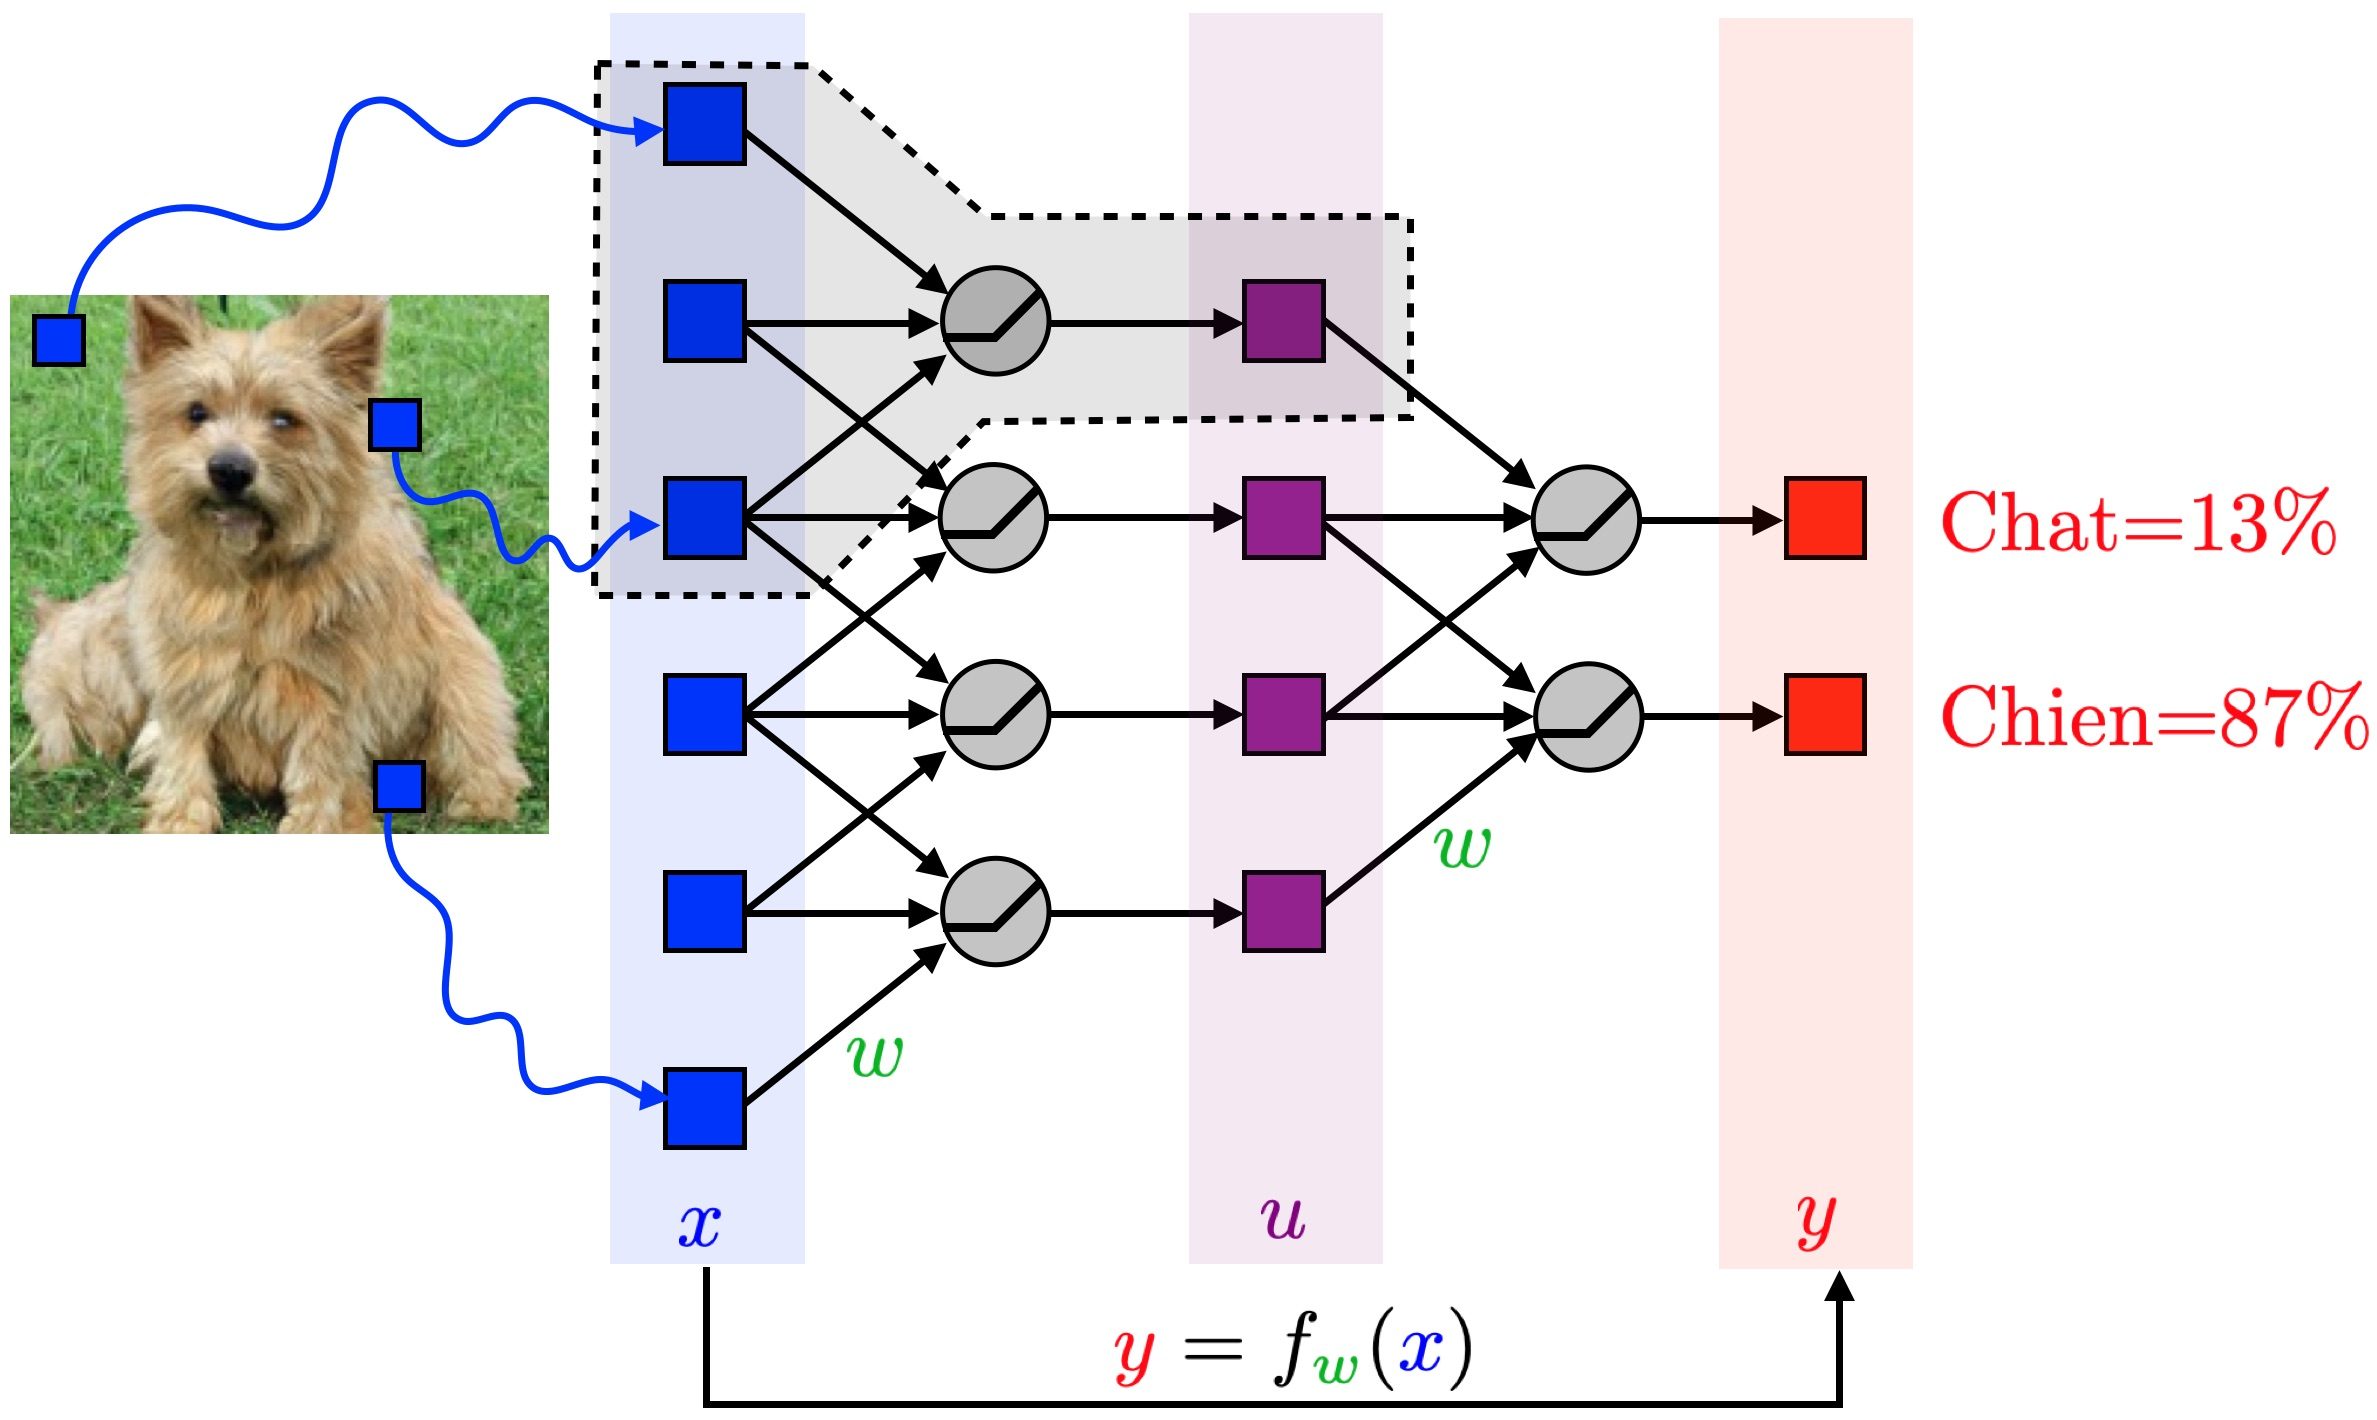
\includegraphics[width=.85\linewidth]{discriminative.jpg}
\caption{Schéma d'un classifieur avec une couche cachée et une couche de sortie. Seuls quelques pixels d'entrée et quelques connexions sont dessinés. Les pourcentages sont des prédictions du modèle ; une normalisation telle que softmax est nécessaire pour obtenir des probabilités de classes.}\label{fig:discriminative}
\end{figure}

Chaque couche associe des opérations affines à une fonction d'activation. Une unité linéaire rectifiée, ou ReLU, calcule
\begin{equation}\label{eq-neuron}
 u_1=\operatorname{ReLU}(w_1x_1+w_2x_2+w_3x_3+b),
 \qquad \operatorname{ReLU}(t)=\max(t,0).
\end{equation}
Les poids déterminent la contribution de chaque entrée ; le biais $b$ déplace le seuil d'activation. Une ReLU renvoie zéro pour une entrée négative ou nulle et conserve les entrées positives. Elle diffère d'un neurone à seuil binaire, qui n'a que deux valeurs de sortie possibles.

\begin{figure}[htbp]\centering
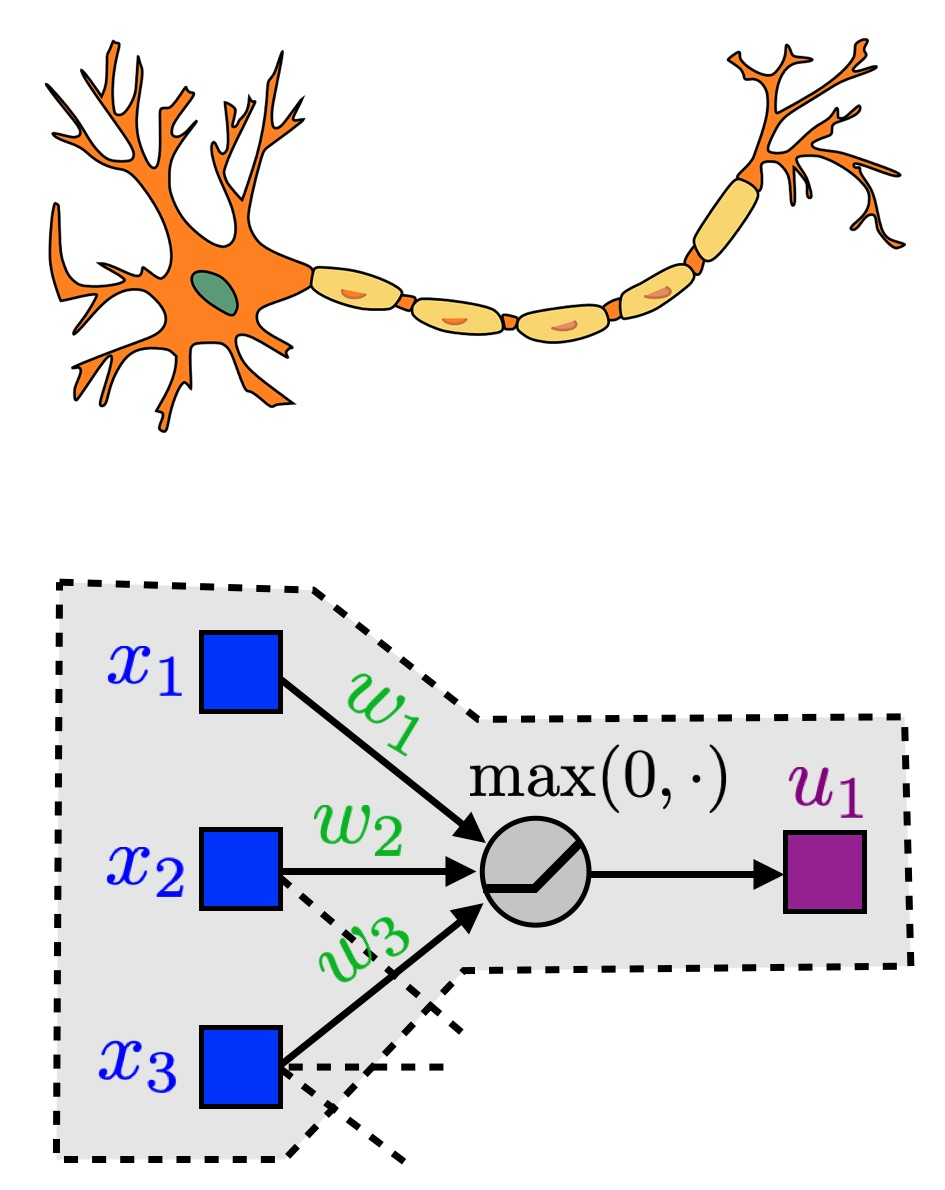
\includegraphics[width=.30\linewidth]{neuron.jpg}
\caption{Un neurone biologique et un neurone artificiel schématique. Le modèle mathématique ne conserve qu'une somme pondérée et une activation ; le biais de~\eqref{eq-neuron} est omis du dessin.}\label{fig:neuron}
\end{figure}

Pour une entrée $x\in\RR^d$, une couche cachée de largeur $m$ et $K$ classes, on peut définir le réseau
\[
 u=\operatorname{ReLU}(Wx+b),\qquad a=Vu+c,\qquad
 \hat y_k=\frac{e^{a_k}}{\sum_{j=1}^K e^{a_j}},
\]
où $W\in\RR^{m\times d}$, $b\in\RR^m$, $V\in\RR^{K\times m}$ et $c\in\RR^K$. ReLU agit coordonnée par coordonnée. L'opération finale est softmax ; les valeurs intermédiaires $a_k$ sont appelées \emph{logits}. En calcul numérique, remplacer chaque $a_k$ par $a_k-\max_j a_j$ donne les mêmes probabilités et évite les débordements. Les entrées de $W,b,V,c$ forment le vecteur de paramètres $w$.

Composer davantage de couches donne un réseau profond. Les activations non linéaires sont essentielles : une composition d'applications affines reste affine. La profondeur permet de représenter certaines fonctions plus économiquement qu'une seule couche cachée très large, mais l'architecture appropriée dépend de la tâche.

Le vocabulaire biologique exprime une analogie, et non un modèle fidèle du cerveau. McCulloch et Pitts ont étudié des neurones logiques à seuil~\cite{mcculloch1943logical}, tandis que le perceptron de Rosenblatt a introduit un premier modèle d'apprentissage~\cite{rosenblatt1957perceptron}. Ces modèles se distinguent des réseaux ReLU décrits ici. Les études biologiques du cortex visuel et de la dynamique membranaire portent sur des mécanismes bien plus riches~\cite{hubel1962receptive,hodgkin1952quantitative}.

\subsection{Apprendre à partir d'exemples étiquetés}
L'apprentissage supervisé part de couples $(x_i,y_i)_{i=1}^n$. Pour une étiquette de classe unique $k_i$, la cible est souvent un vecteur indicateur : $(y_i)_{k_i}=1$, et toutes les autres composantes sont nulles. Ces étiquettes représentent des annotations, plutôt que des probabilités conditionnelles connues. Les données peuvent provenir d'annotations humaines ou d'une autre source de supervision, et contenir des erreurs.

\begin{figure}[htbp]\centering
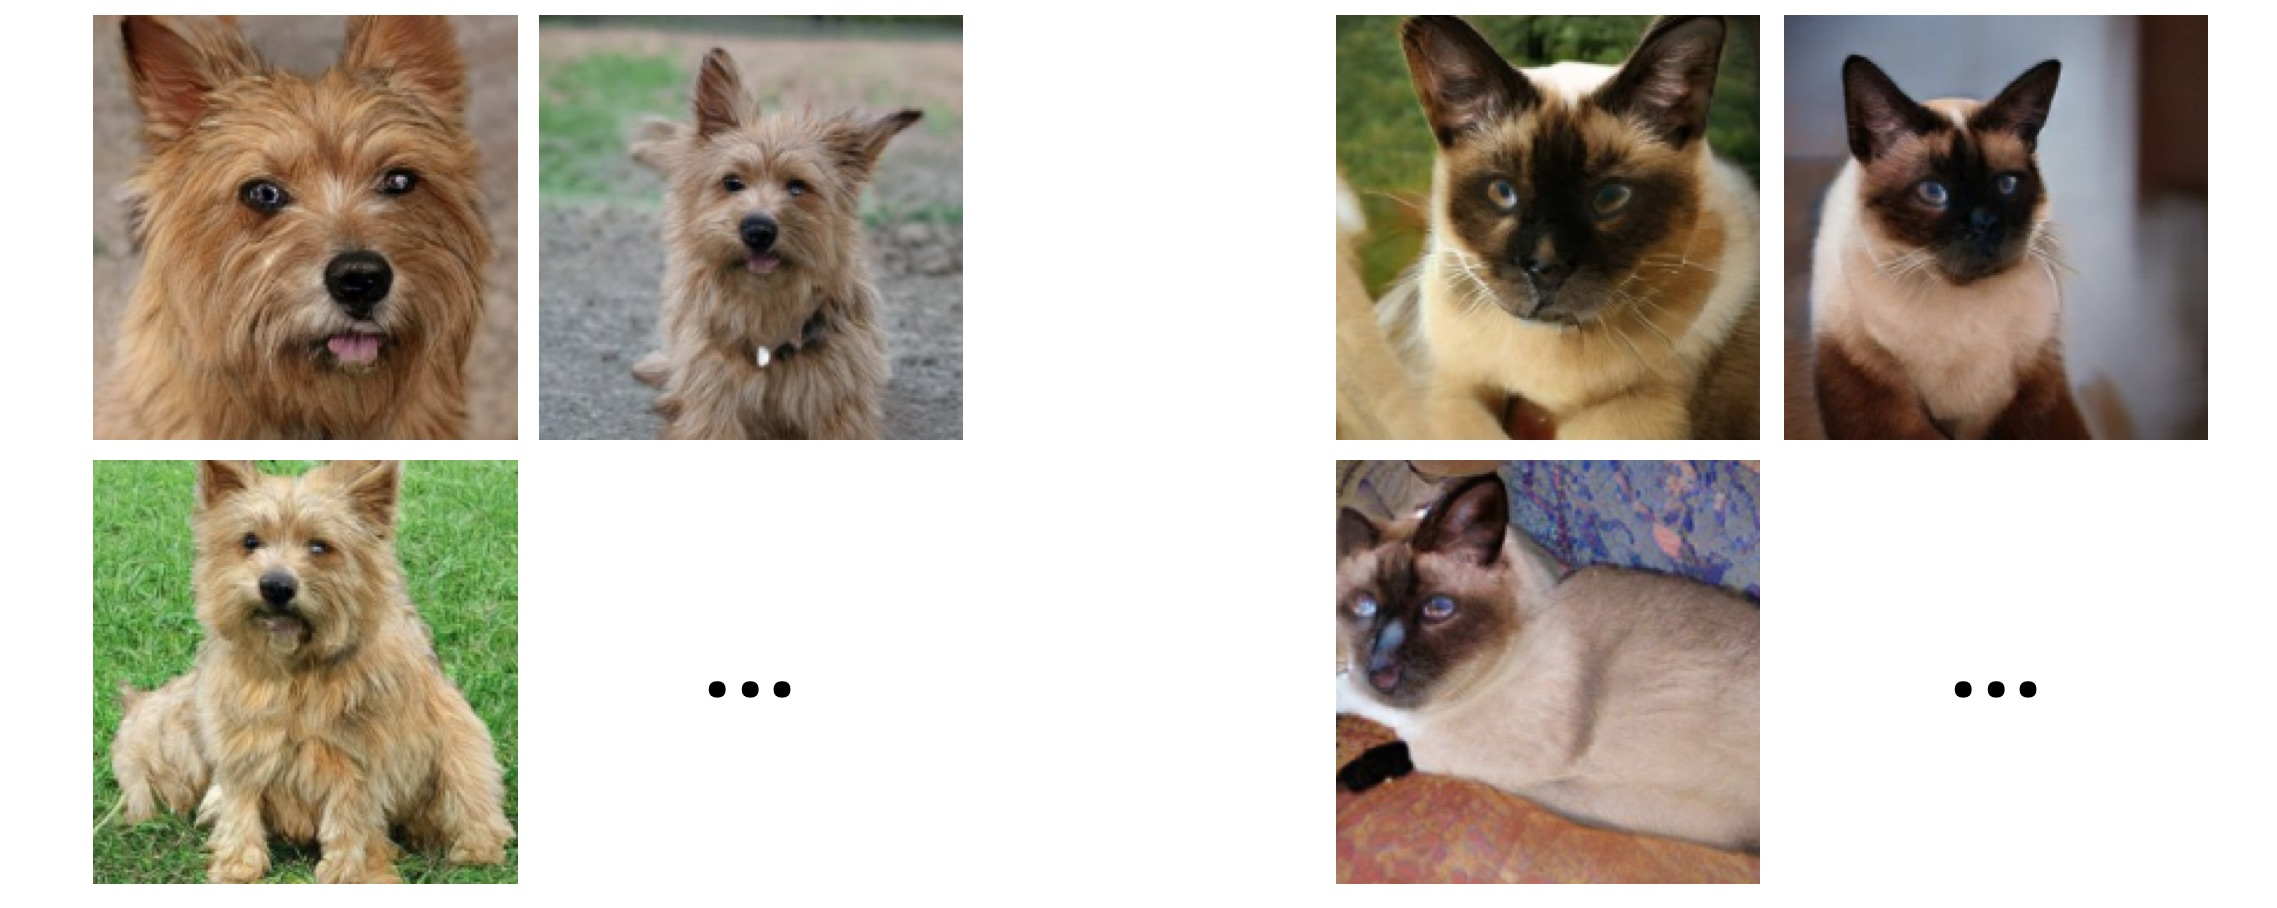
\includegraphics[width=.82\linewidth]{dataset.jpg}
\caption{Exemples d'images étiquetées de chiens et de chats issues d'ImageNet~\cite{deng2009imagenet}. L'apprentissage utilise de nombreux exemples ; l'évaluation demande des données séparées.}\label{fig:dataset}
\end{figure}

L'objectif d'apprentissage mesure le désaccord entre prédictions et étiquettes. L'erreur quadratique moyenne et l'entropie croisée en sont deux exemples :
\begin{align}
 E_{\mathrm{sq}}(w)&=\frac1n\sum_{i=1}^n\norm{f_w(x_i)-y_i}_2^2,\label{eq-nn-square}\\
 E_{\mathrm{CE}}(w)&=-\frac1n\sum_{i=1}^n\sum_{k=1}^K(y_i)_k\log(f_w(x_i)_k).
 \label{eq-nn-ce}
\end{align}
Pour une cible indicatrice, le terme d'entropie croisée correspondant vaut $-\log(f_w(x_i)_{k_i})$. Le logarithme est naturel, et softmax donne des probabilités strictement positives pour des logits finis. Une implémentation stable évalue directement le logarithme de softmax. On peut ajouter à l'objectif une pénalité sur les poids.

L'entraînement cherche à réduire cette erreur empirique. Comme le réseau dépend non linéairement de nombreux paramètres, l'objectif est généralement non convexe. Les méthodes d'optimisation peuvent être efficaces sans fournir de garantie générale d'atteindre son minimum global.

\subsection{Rétropropagation et mise à jour des poids}
La rétropropagation calcule le gradient d'une perte scalaire en appliquant la règle de dérivation des fonctions composées à travers le réseau, dans l'ordre inverse~\cite{rumelhart1986learning,linnainmaa1976taylor}. C'est la différentiation automatique en mode inverse. Un algorithme d'optimisation utilise ensuite ces dérivées pour mettre à jour les poids ; par exemple, la descente de gradient effectue le pas
\[
 w^{(t+1)}=w^{(t)}-\eta_t\nabla E(w^{(t)}),\qquad \eta_t>0.
\]
Le choix du pas est important : un pas trop grand peut augmenter l'erreur. La descente de gradient stochastique remplace le gradient complet par une estimation calculée sur un petit lot choisi aléatoirement, ce qui réduit le coût de chaque mise à jour. Un pas stochastique individuel ne diminue pas nécessairement l'erreur totale d'apprentissage.

Pour le classifieur à deux couches ci-dessus et un exemple de perte $\ell$ donnée par l'entropie croisée, la dérivation se lit directement. Posons $r=Wx+b$, $u=\operatorname{ReLU}(r)$ et $\delta=\hat y-y$. En dehors des points où $r_j=0$,
\[
 \frac{\partial\ell}{\partial V}=\delta u^\mathsf{T},\qquad
 \frac{\partial\ell}{\partial c}=\delta,\qquad
 q=(V^\mathsf{T}\delta)\odot\mathbf1_{r>0},\qquad
 \frac{\partial\ell}{\partial W}=qx^\mathsf{T},\quad
 \frac{\partial\ell}{\partial b}=q.
\]
Le symbole $\odot$ désigne le produit coordonnée par coordonnée. Au point anguleux de ReLU, les logiciels choisissent une convention, souvent zéro, pour la dérivée de l'activation. Cette convention ne rend pas le réseau différentiable au sens classique en ce point.

De grandes bases étiquetées, le calcul efficace sur processeurs graphiques et les progrès des architectures et de l'entraînement ont contribué au succès des classifieurs profonds, notamment au résultat ImageNet de 2012~\cite{krizhevsky2012imagenet}. Des techniques de régularisation comme le \emph{dropout} peuvent limiter le surapprentissage~\cite{srivastava2014dropout}. Les travaux de Yoshua Bengio, Geoffrey Hinton et Yann LeCun ont été distingués par le prix Turing 2018 de l'ACM, annoncé en 2019.\footnote{\url{https://awards.acm.org/about/2018-turing}}

\subsection{Approximation, optimisation et généralisation}
Un théorème d'approximation universelle porte sur ce qu'un réseau peut représenter. Un résultat classique de Cybenko~\cite{cybenko1989approximation} affirme que, pour une fonction continue $F:[0,1]^d\to\RR$ et tout $\varepsilon>0$, il existe un entier fini $m$ et des coefficients tels que
\[
 G(x)=\sum_{j=1}^m\alpha_j\sigma(v_j\cdot x+\beta_j),
 \qquad \sup_{x\in[0,1]^d}|F(x)-G(x)|<\varepsilon,
\]
où $\sigma$ est une activation sigmoïde continue fixée, par exemple $\sigma(t)=1/(1+e^{-t})$. La couche de sortie est linéaire, et la largeur et les poids ne sont pas contraints. Il s'agit du théorème pour les sigmoïdes ; les résultats d'approximation pour les réseaux ReLU demandent leurs propres énoncés.

Ce théorème ne fait intervenir aucune donnée d'apprentissage. Il n'exige pas une infinité d'exemples et ne garantit pas qu'un algorithme puisse trouver le réseau approchant à partir d'un nombre fini d'observations. Trois questions doivent être distinguées : l'existence d'une bonne représentation, la capacité de l'optimisation à la trouver et la qualité des prédictions sur de nouvelles données.

La généralisation s'évalue sur des données exclues de l'entraînement. Les données de validation guident des choix comme l'architecture et le moment d'arrêt ; un jeu de test distinct évalue la procédure finale. La qualité des résultats dépend aussi de la représentativité de ces données par rapport aux conditions d'utilisation du réseau.

Les réseaux convolutifs intègrent des hypothèses sur la structure spatiale~\cite{lecun1998gradient}. Les connexions locales limitent le champ réceptif, et le partage des poids applique le même filtre en différentes positions. Une convolution de pas un commute avec les translations sur une grille infinie ou périodique ; les conditions au bord et le sous-échantillonnage peuvent modifier cette propriété. L'équivariance par translation d'une carte de caractéristiques se distingue également de l'invariance par translation d'une classification finale.

L'architecture, la régularisation, les données et l'optimisation influencent toutes les performances~\cite{lecun2015deep}. Des résultats mathématiques expliquent certains mécanismes et certains régimes, mais aucun théorème unique ne rend compte de toutes les architectures efficaces.
